%!TEX TS-program = xelatex
\documentclass[]{friggeri-cv}
\usepackage{graphicx}
\usepackage[spanish]{babel}
\addbibresource{bibliography.bib}
\begin{document}
\header{Francisco Rafael }{Arce García}
       {Administrador de TI \& Desarrollador Junior}
% In the aside, each new line forces a line break
\begin{aside}
  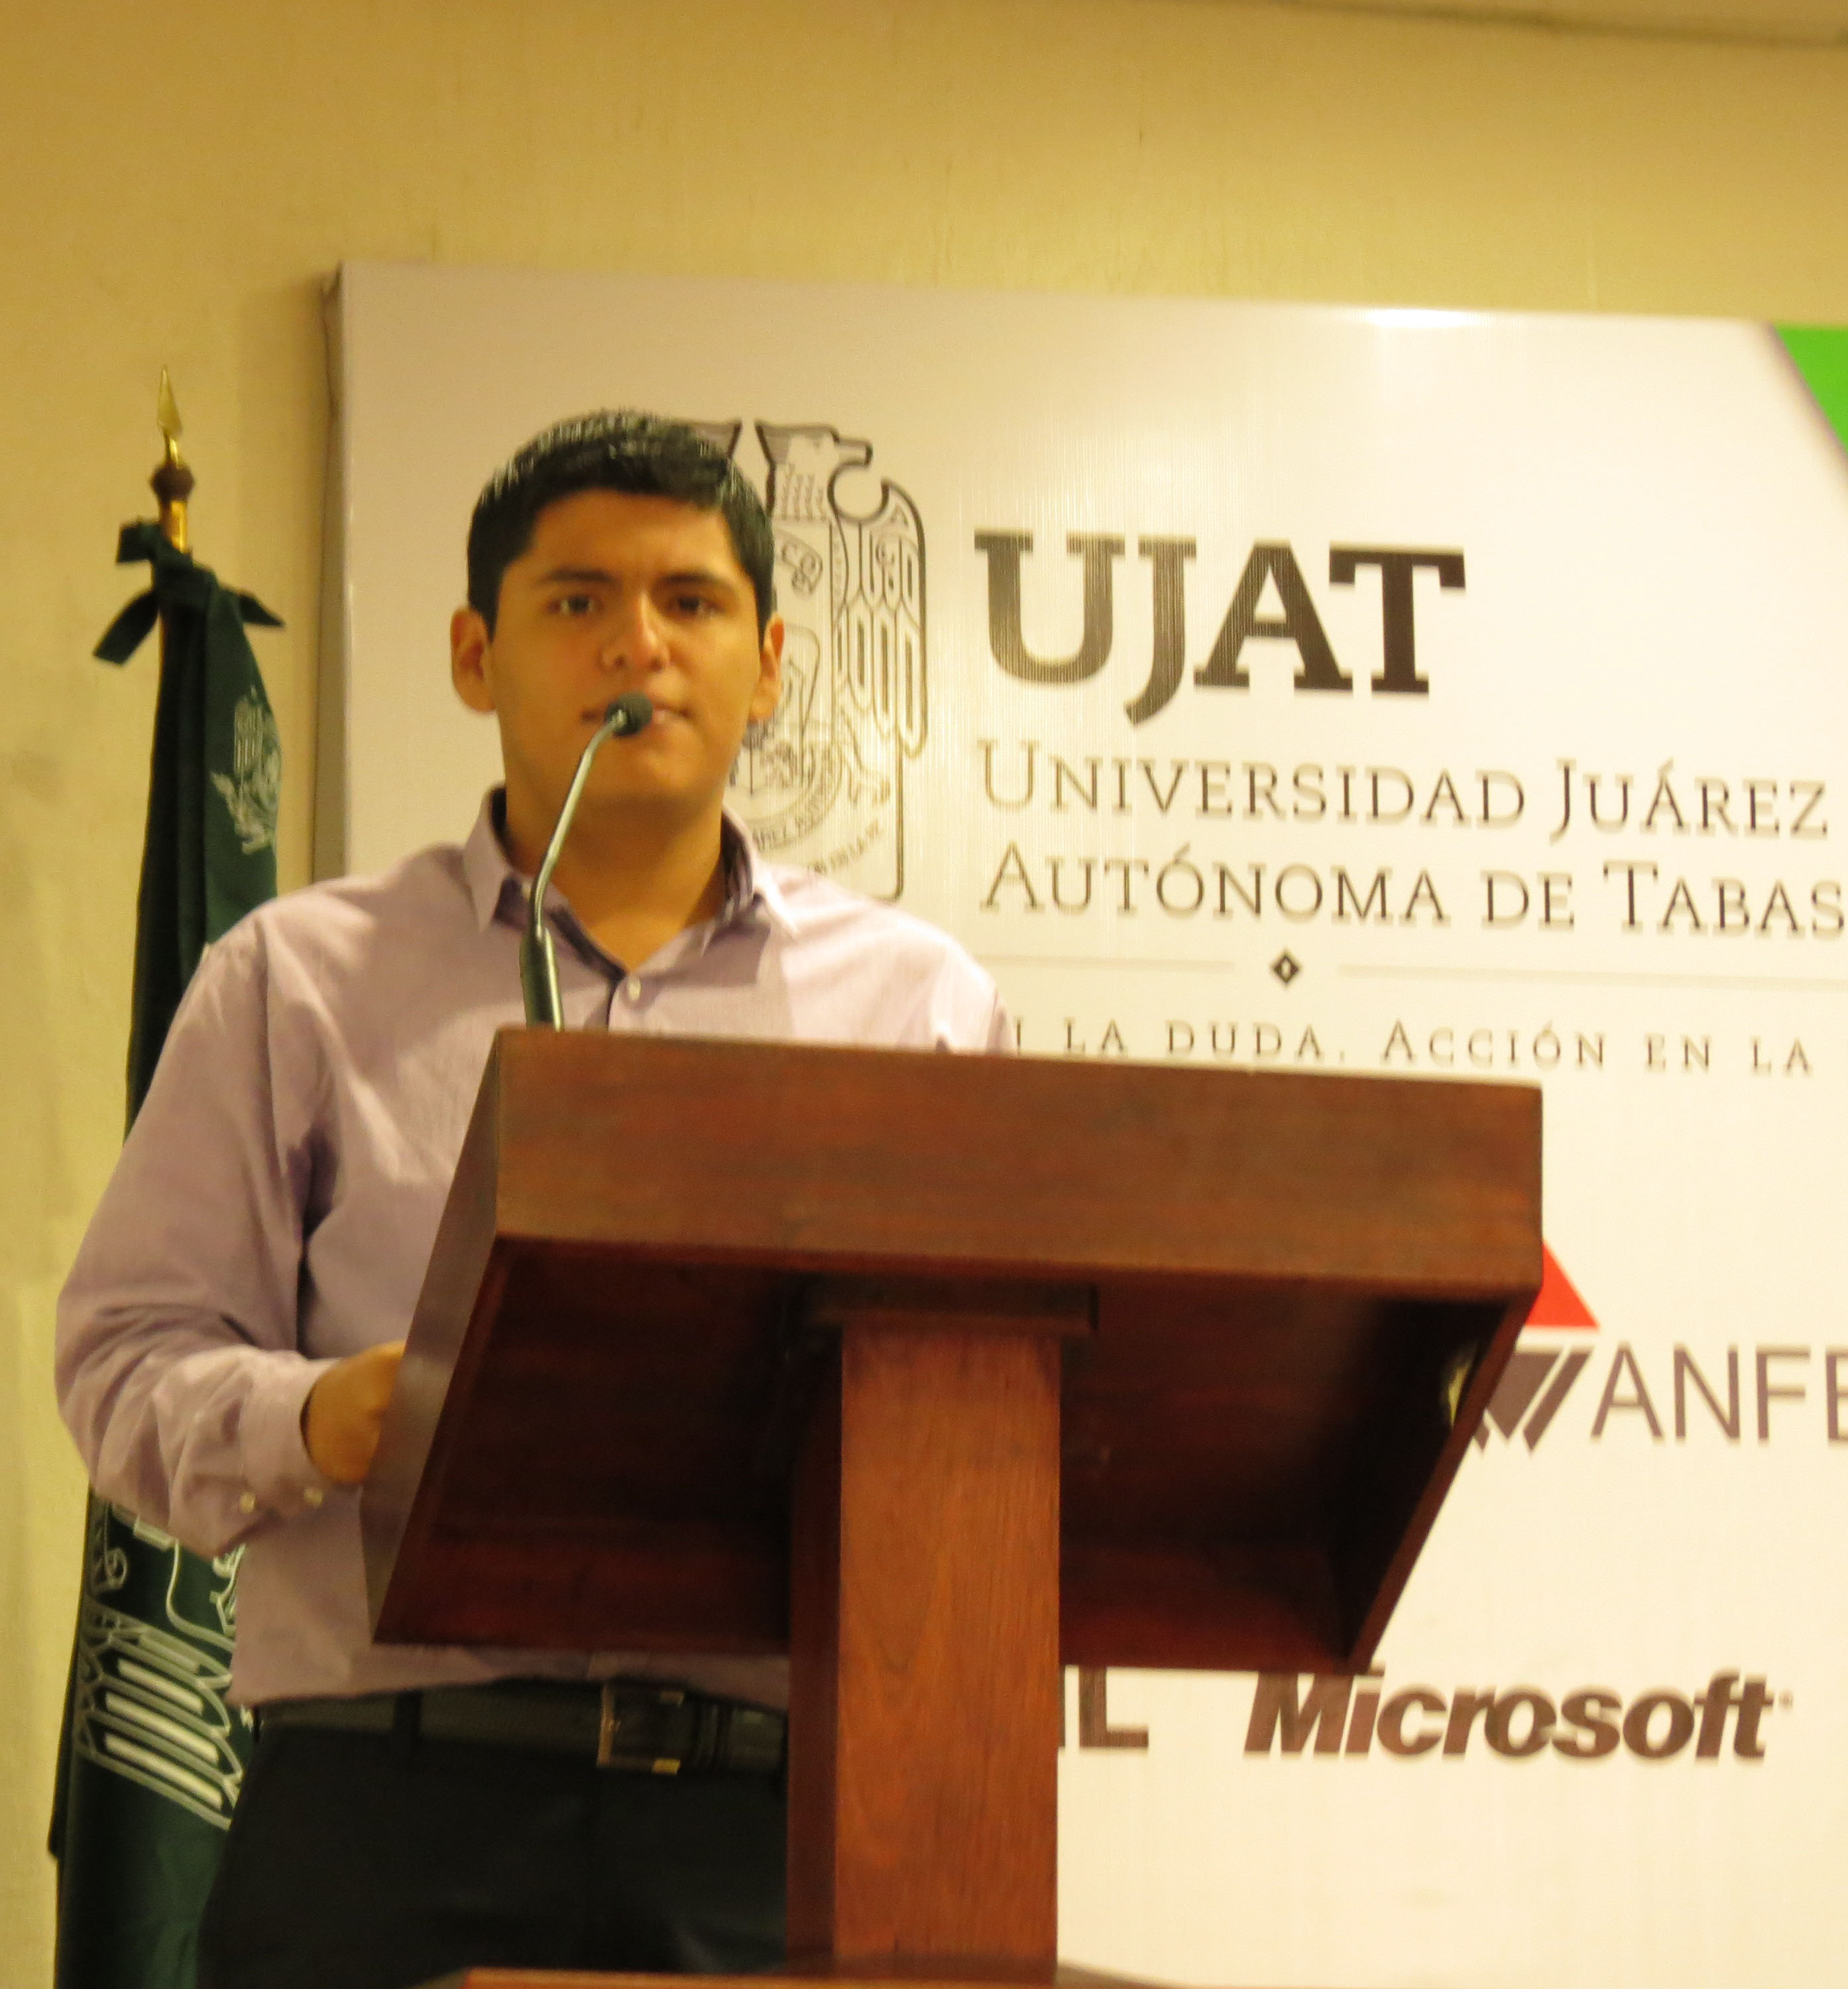
\includegraphics[scale=0.08]{yo}
  \section{Acerca}
    Tepotzotlán
    Estado de México,
    México
    ~
    \href{mailto:fragmnt02@gmail.com}{fragmnt02@gmail.com}
    \href{https://www.linkedin.com/in/franciscorafaelarcegarcia}{LinkedIn (Clic Aquí)}
    \href{https://github.com/fragmnt02}{Github: fragmnt02}
  \section{Idiomas}
    Ingles (Profesional)
    Español (Nativo)
  \section{Programación}
    Java
    Javascript
    (node.js, express.js)
    SQL
    (SQL Server, MySQL)
    HTML5 \& CSS3
    LaTeX
  \section{Marketing Digital}
    Google Adwords
    Google Analytics
    Facebook Ads
    Twitter Ads
  \section{Otras Herramientas}
    Microsoft Office
    Adobe Photoshop
    Adobe After Effects
    Sony Vegas Pro
    Cisco CLI
\end{aside}
\section{Intereses}
Egresado con honores de la Licenciatura en Telemática en busca de oportunidades para desarrollarse en el mercado laboral actual de las tecnologías de la información y el marketing digital.
\section{Educación}
\begin{entrylist}
  \entry
    {2013-2017}
    {Licenciatura en Telemática}
    {Universidad Juárez Autónoma de Tabasco (UJAT).}
    {Calificación: 9.7}
  \entry
    {2016-2017}
    {Alumno de Intercambio}
    {Universidad de Salamanca, España.}
    {Calificación: 8.5}
\end{entrylist}
\section{Experiencia}
\begin{entrylist}
  \entry
    {05–08 2016}
    {Asistente de Investigación}
    {Latin American Summer Research Program.}
    {\emph{University of Arizona - Eller College of Management, Arizona, E.U.A.}}
  \entry
    {02–07 2017}
    {Administrador de TI}
    {Becario/Practicas Profesionales.}
    {\emph{Escuela Telesecundaria “Rosendo Taracena Padrón”.}}
\end{entrylist}
\section{Voluntariado}
\begin{entrylist}
  \entry
    {2014}
    {Mentor de Estudiantes}
    {Universidad Juárez Autónoma de Tabasco.}
    {Asesoría a estudiantes para procedimientos escolares en la universidad y mentorías académicas.}
  \entry
    {2015}
    {Organizador de Comunidades sin Ánimo de Lucro}
    {DevCunduacán.}
    {DevCunduacán es un conjunto de conferencias y talleres impartidas al público en general donde se impulsa el emprendimiento y uso de nuevas tecnologías.}
\end{entrylist}
\section{Certificaciones}
\begin{entrylist}
    \entry{2016}
          {TOEFL IBT}
          {ETS}
          {Fecha de Expiración: Febrero, 2018.}
    \entry{2018}
          {Adwords Fundamentals}
          {Google}
          {Fecha de Expiración: Febrero, 2019.}
    \entry{2018}
          {Adwords Mobile}
          {Google}
          {Fecha de Expiración: Febrero, 2019.}
    \entry{2018}
          {Marketing Leadership}
          {Twitter}
          {Sin Fecha de Expiración}
\end{entrylist}
\newline
\newline
\newline
\newline
\newline
\section{Copyright}
\begin{entrylist}
    \entry{2017}
          {Software: “Estilos de Aprendizaje - UJAT”}
          {UJAT}
          {Aplicación web para determinar el estilo de aprendizaje predominante en un grupo de alumnos. Este proyecto fue desarrollado mediante la aplicación de tecnologías como Node.js, Express.js, Jade y Google Charts.}
\end{entrylist}
\section{Publicaciones}
\begin{entrylist}
    \entry{2016}
          {Articulo: Metaheurísticas en Dispositivos Móviles. Caso: Rutas de Mapas}
          {UJAT}
          {Colección de Avances en Tecnologías de la Información, Volumen II. }
    \entry{2016}
          {Articulo: Simplificación de Textos Médicos Mediante Procesamiento de Lenguaje Natural}
          {UJAT}
          {Perspectiva Científica de la UJAT, Volumen V.}
    \entry{2017}
          {Tesis: Rutas de Mapas para Dispositivos Móviles a través de Metaeurística}
          {UJAT}
          {Tesis para la obtención de título como licenciado en Telemática.}    
\end{entrylist}
\section{Reconocimientos y Premios}
\begin{entrylist}
    \entry{2013}
          {Segundo Lugar en "Rally de Conocimientos"}
          {DAIS}
          {Segundo lugar en el rally de conocimientos en el marco del 10 Congreso Nacional y 7 Internacional de Informática y Sistemas.}
    \entry{2014}
          {Estudiante de Alto Rendimiento Académico en el periodo Agosto, 2013 y Febrero, 2014.}
          {DAIS}
          {}
    \entry{2014}
          {Estudiante de Alto Rendimiento Académico en el periodo Febero y Agosto del 2014.}
          {DAIS}
          {}
    \entry{2015}
          {Estudiante de Alto Rendimiento Académico en el periodo Agosto, 2014 y Enero, 2015.}
          {DAIS}
          {}
    \entry{2015}
          {Estudiante de Alto Rendimiento Académico en el periodo Febrero y Agosto del 2015.}
          {DAIS}
          {}
    \entry{2017}
          {Mejor Promedio de la Generación 2012 - 2017}
          {UJAT}
          {Reconocimiento por haber obtenido 9.79, el promedio mas alto de la generación 2012 - 2017.}
    \entry{2017}
          {Mejor Promedio de la Licenciatura en Telemática}
          {UJAT}
          {Generación 2013 - 2017.}
    \entry{2017}
          {Medalla "Manuel Sánchez Mármol"}
          {UJAT}
          {Medalla para estudiantes con alto rendimiento académico.}
\end{entrylist}
\newline
\newline
\newline
\newline
\newline
\newline
\newline
\section{Cursos}
\begin{entrylist}
    \entry{2013}
          {Taller de Tendencias Tecnológicas IBM.}
          { 10 Congreso Nacional y 7 Internacional de Informática y Sistemas}
          {}
    \entry{2013}
          {Seminario de Aplicaciones Móviles con Tecnología Web.}
          {10 Congreso Nacional y 7 Internacional de Informática y Sistemas}
          {}
    \entry{2014}
          {Ensamble y Mantenimiento de PCs.}
          {Universidad Juárez Autónoma de Tabasco}
          {}
    \entry{2015}
          {Taller de Aplicaciones de Matemáticas Usando Software Geogebra. }
          { Simposio de Matemáticas Aplicadas a Tecnologías de la Información}
          {}
    \entry{2015}
          {Formación de Mentores.}
          {Programa de Mentoría de Estudiantes en la UJAT}
          {}
    \entry{2015}
          {Taller de Django.}
          {12 Congreso Nacional y 9 Internacional de Informática y Sistemas}
          {}
    \entry{2016}
          {Talleres en University of Arizona:}
          {Latin American Summer Research Program}
          {Abstract Workshop, Scientific Poster Workshop, Purpose/Personal Statement Workshop y Oral Presentation Workshop}
    \entry{2016}
          {Fundamentos de Marketing Online.}
          {Google}
          {}
    \entry{2018}
          {Marca Personal.}
          {Platzi}
          {}
\end{entrylist}
\newline
\newline
\newline
\newline
\newline
\newline
\newline
\newline
\newline
\newline
\newline
\newline
\newline
\newline
\newline
\newline
\newline
\newline
\newline
\newline
\newline
\newline
\newline
\newline
Para cualquier duda, comentario o documento de soporte, no dude en comunicarse.\\
Última Actualización: \today
%%% This piece of code has been commented by Karol Kozioł due to biblatex errors. 
% 
%\printbibsection{article}{article in peer-reviewed journal}
%\begin{refsection}
%  \nocite{*}
%  \printbibliography[sorting=chronological, type=inproceedings, title={international peer-reviewed conferences/proceedings}, notkeyword={france}, heading=subbibliography]
%\end{refsection}
%\begin{refsection}
%  \nocite{*}
%  \printbibliography[sorting=chronological, type=inproceedings, title={local peer-reviewed conferences/proceedings}, keyword={france}, heading=subbibliography]
%\end{refsection}
%\printbibsection{misc}{other publications}
%\printbibsection{report}{research reports}

\end{document}
